\documentclass[conference]{IEEEtran}


\usepackage{booktabs} % format tables
\usepackage{times} % times font can reduce page length
\usepackage{color} % color figures
\usepackage{balance} %balance the end of the draft
\usepackage{url}
%\usepackage[all]{nowidow}
\usepackage{tabularx}
\usepackage{siunitx} %unit package for special unit symbols
\usepackage{epsfig,tabularx,subfigure,multirow, graphicx}
\let\labelindent\relax
\usepackage{enumitem}
%\usepackage[sorting=none]{biblatex}
\usepackage{caption}
\captionsetup[figure]{font=small,skip=0ex, belowskip=-2ex}
\captionsetup[table]{font=small,skip=0ex, belowskip=-4ex}


\usepackage{hyperref} % add hyper reference to citations and references

\let\proof\relax
\let\endproof\relax
\usepackage{amsthm,amssymb,amsmath}  % support for mathematic symbols

\newcolumntype{L}[1]{>{\raggedright\arraybackslash}p{#1}}
\newcolumntype{C}[1]{>{\centering\arraybackslash}p{#1}}
\newcolumntype{R}[1]{>{\raggedleft\arraybackslash}p{#1}}

\usepackage[linesnumbered,ruled,vlined]{algorithm2e}
\usepackage{etoolbox}
%%%%%%%%%%%%%%%%%%%%%%%%%%%%A patch to remove right margin in algorithm2e block
\makeatletter
% Remove right hand margin in algorithm
\patchcmd{\@algocf@start}% <cmd>
{-1.5em}% <search>
{0pt}% <replace>
{}{}% <success><failure>
\makeatother
%%%%%%%%%%%%%%%%%%%%%%%%%%%%%%%%%

%%%%%%%%%%%%%%set font in algorithms smaller
\SetAlFnt{\small}
\SetAlCapFnt{\small}
\SetAlCapNameFnt{\small}
\usepackage{algorithmic}
\algsetup{linenosize=\tiny}
%%%%%%%%%%%%%%%%%%%%%%%%%%%%%%%

\SetKwRepeat{Do}{do}{while}% add do-while sentences
\newcommand\mycommfont[1]{\scriptsize\ttfamily{#1}} %adjust the font size of comments
\SetCommentSty{mycommfont}


\newcommand{\stitle}[1]{\vspace{1ex} \noindent{\bf #1}}
\long\def\comment#1{}

\setlength{\algomargin}{1em} %adjust the side margin of algorithm blocks
%\setlength{\textfloatsep}{1ex} %adjust the space above and below the float block, including algorithms, figures, tables

\DeclareMathOperator*{\argmin}{arg\,min}

\newcommand{\nop}[1]{}

\newcommand{\figureTopMargin}{\vspace{-3ex}}
\newcommand{\figureCaptionMargin}{\vspace{-2ex}}
\newcommand{\figureBelowMargin}{\vspace{-2ex}}
\newcommand{\tableTopMargin}{\vspace{-4ex}}
\newcommand{\tableBelowMargin}{\vspace{-3ex}}
\newcommand{\algoTopMargin}{\vspace{-3ex}}
\newcommand{\algoBelowMargin}{\vspace{-3ex}}
\newcommand{\itemMargin}{\vspace{-1ex}}

\newcommand\abs[1]{\left\lvert #1 \right\rvert}


%%%%%%%uncomment below commands to enable related blocks
\newtheorem{theorem}{\bf Theorem}[section]
\newtheorem{lemma}{\bf Lemma}[section]
\newtheorem{corollary}{\bf Corollary}[section]
\newtheorem{example}{\bf Example}

\theoremstyle{remark}
\newtheorem{remark}{\bf Remark}[section]

\theoremstyle{definition}
\newtheorem{definition}{\bf Definition}




\title{Crowdrebate: An Effective Platform to Getting more Rebate for Customers}

\author{
	{Nian Chen{\small $~^{\dagger}$}, Weijie Sun{\small $~^{\dagger}$}, Wangze Ni{\small $~^{\dagger}$}, Zhao Chen{\small $~^{\dagger}$}, Jiale Gu{\small $~^{\dagger}$}, Peng Cheng{\small $~^{*}$}, Lei Chen{\small $~^{\dagger}$}, Xuemin Lin{\small $~^{\#,*}$}
	} \\
	\fontsize{10}{10}\selectfont\itshape
	$~^{\dagger}$The Hong Kong University of Science and Technology, Hong Kong, China\\
	\fontsize{9}{9}\selectfont\ttfamily\upshape
	\{nchenaf, zchenah\}@connect.ust.hk, \{wsunan, wniab, leichen\}@cse.ust.hk, jialgu@ust.hk\\
	\fontsize{10}{10}\selectfont\itshape
	$~^{*}$East China Normal University, Shanghai, China\\
	\fontsize{9}{9}\selectfont\ttfamily\upshape pcheng@sei.ecnu.edu.cn \\
	\fontsize{10}{10}\selectfont\itshape
	$~^{\#}$The University of New South Wales, Australia\\
	\fontsize{9}{9}\selectfont\ttfamily\upshape
	lxue@cse.unsw.edu.au\\
	%\fontsize{10}{10}\selectfont\itshape
	%$~^{\ddagger}$ Shenzhen Onething Technologies Co., Ltd., Shenzhen, China\\
	%\fontsize{9}{9}\selectfont\ttfamily\upshape
	%\{leichen, laixin, zhangxiao\}@onething.net \\
}

%\numberofauthors{4}
%\author{
%	\alignauthor Nian CHEN \\
%	\affaddr{Hong Kong university of science and technology} \\
%	\affaddr{Hong Kong, China} \\
%	\affaddr{nchenaf@connect.ust.hk}
%	\alignauthor Nian Chen \\
%	\affaddr{Hong Kong university of science and technology} \\
%	\affaddr{Hong Kong, China} \\
%	\affaddr{nchenaf@connect.ust.hk}
%	\alignauthor Peng Cheng \\
%	\affaddr{East China Normal University} \\
%		\affaddr{Shang Hai, China} \\
%	\affaddr{pcheng@sei.ecnu.edu.cn}
%		\alignauthor Lei Chen \\
%	\affaddr{Hong Kong university of science and technology} \\
%	\affaddr{Hong Kong, China} \\
%	\affaddr{leichen@cse.ust.hk }
%}



\begin{document}
\maketitle

\begin{abstract}
With the flourishing development of e-commerce platforms, there are various promotion operations, such as offering coupons with a high threshold to stimulate customers to buy more products all at once. Nevertheless, customers always find that the price of the products they intend to order is below the coupons or free delivery service threshold. In order to enjoy these instant benefits, they often need to spend a lot of time looking for others with the same need to place an order together.

In order to address the above issues, we develop a Crowdrebate platform that collects users' requests and groups them into a set of orders qualifying to use the suitable coupons by the Crowdrebate algorithm, after that, Crowdrebate delivers products to different receivers in an order, aiming at saving users' shopping time and helping users get more rebate from online promotions. Crowdrebate is equipped with several novel techniques, including the Crowdrebate algorithm grouping orders for maximum instant rebates, web crawling, items recommendation, and data visualization. We introduce the sketch of the system architecture of Crowdrebate and demonstrate various scenarios via several case analyses. 
\end{abstract}
\section{Introduction}

With the flourishing development of e-commerce platforms, online shopping has become part of people's lives. In order to further stimulate online consumption, e-commerce platforms arrange various promotion campaigns on special days, such as Black Friday~\cite{2013Black} in Western countries and Double Eleven in China~\cite{huang2019x}. Due to the fact that online promotions are too numerous, people can not get promotion information for the first time, some intermediate platforms have emerged in the market, such as Groupon~\cite{groupon} and Dealmoon~\cite{dealmoon}. These platforms help users sort out the hot deals of various e-commerce platforms, saving the user's shopping time.

However, sometimes even users know those promotion, they found that their purchase fails to meet the spending threshold to use a coupon or to enjoy the delivery service. In this situation, users will intentionally ask their friends or look for other person on the social networks to place one order together in order to meet the threshold. Because all the e-commerce platforms support only one shipping address for one order, when multiple users place an order together, one of the users will inevitably receive all the products first and then distribute them to others respectively. These complex processes are unreliable and time-consuming for consumers.

What is even more damaging to consumers' motivation to shopping is that e-commerce promotion activities have become increasingly complicated in recent years. For example, during the 2020 Taobao Double eleven, the platform prolonged the promotional period. This change might aim at bringing more benefits and convenience to consumers, but indeed imposes extra workloads to them, since multiple complex coupons rules change on a daily basis. As a matter of fact, consumers complains that it takes much time to decipher the coupon rules in order to enjoy the event's maximum benefit~\cite{2020} ~\cite{double11}.
\begin{figure}[t] 
\centering %图片居中
		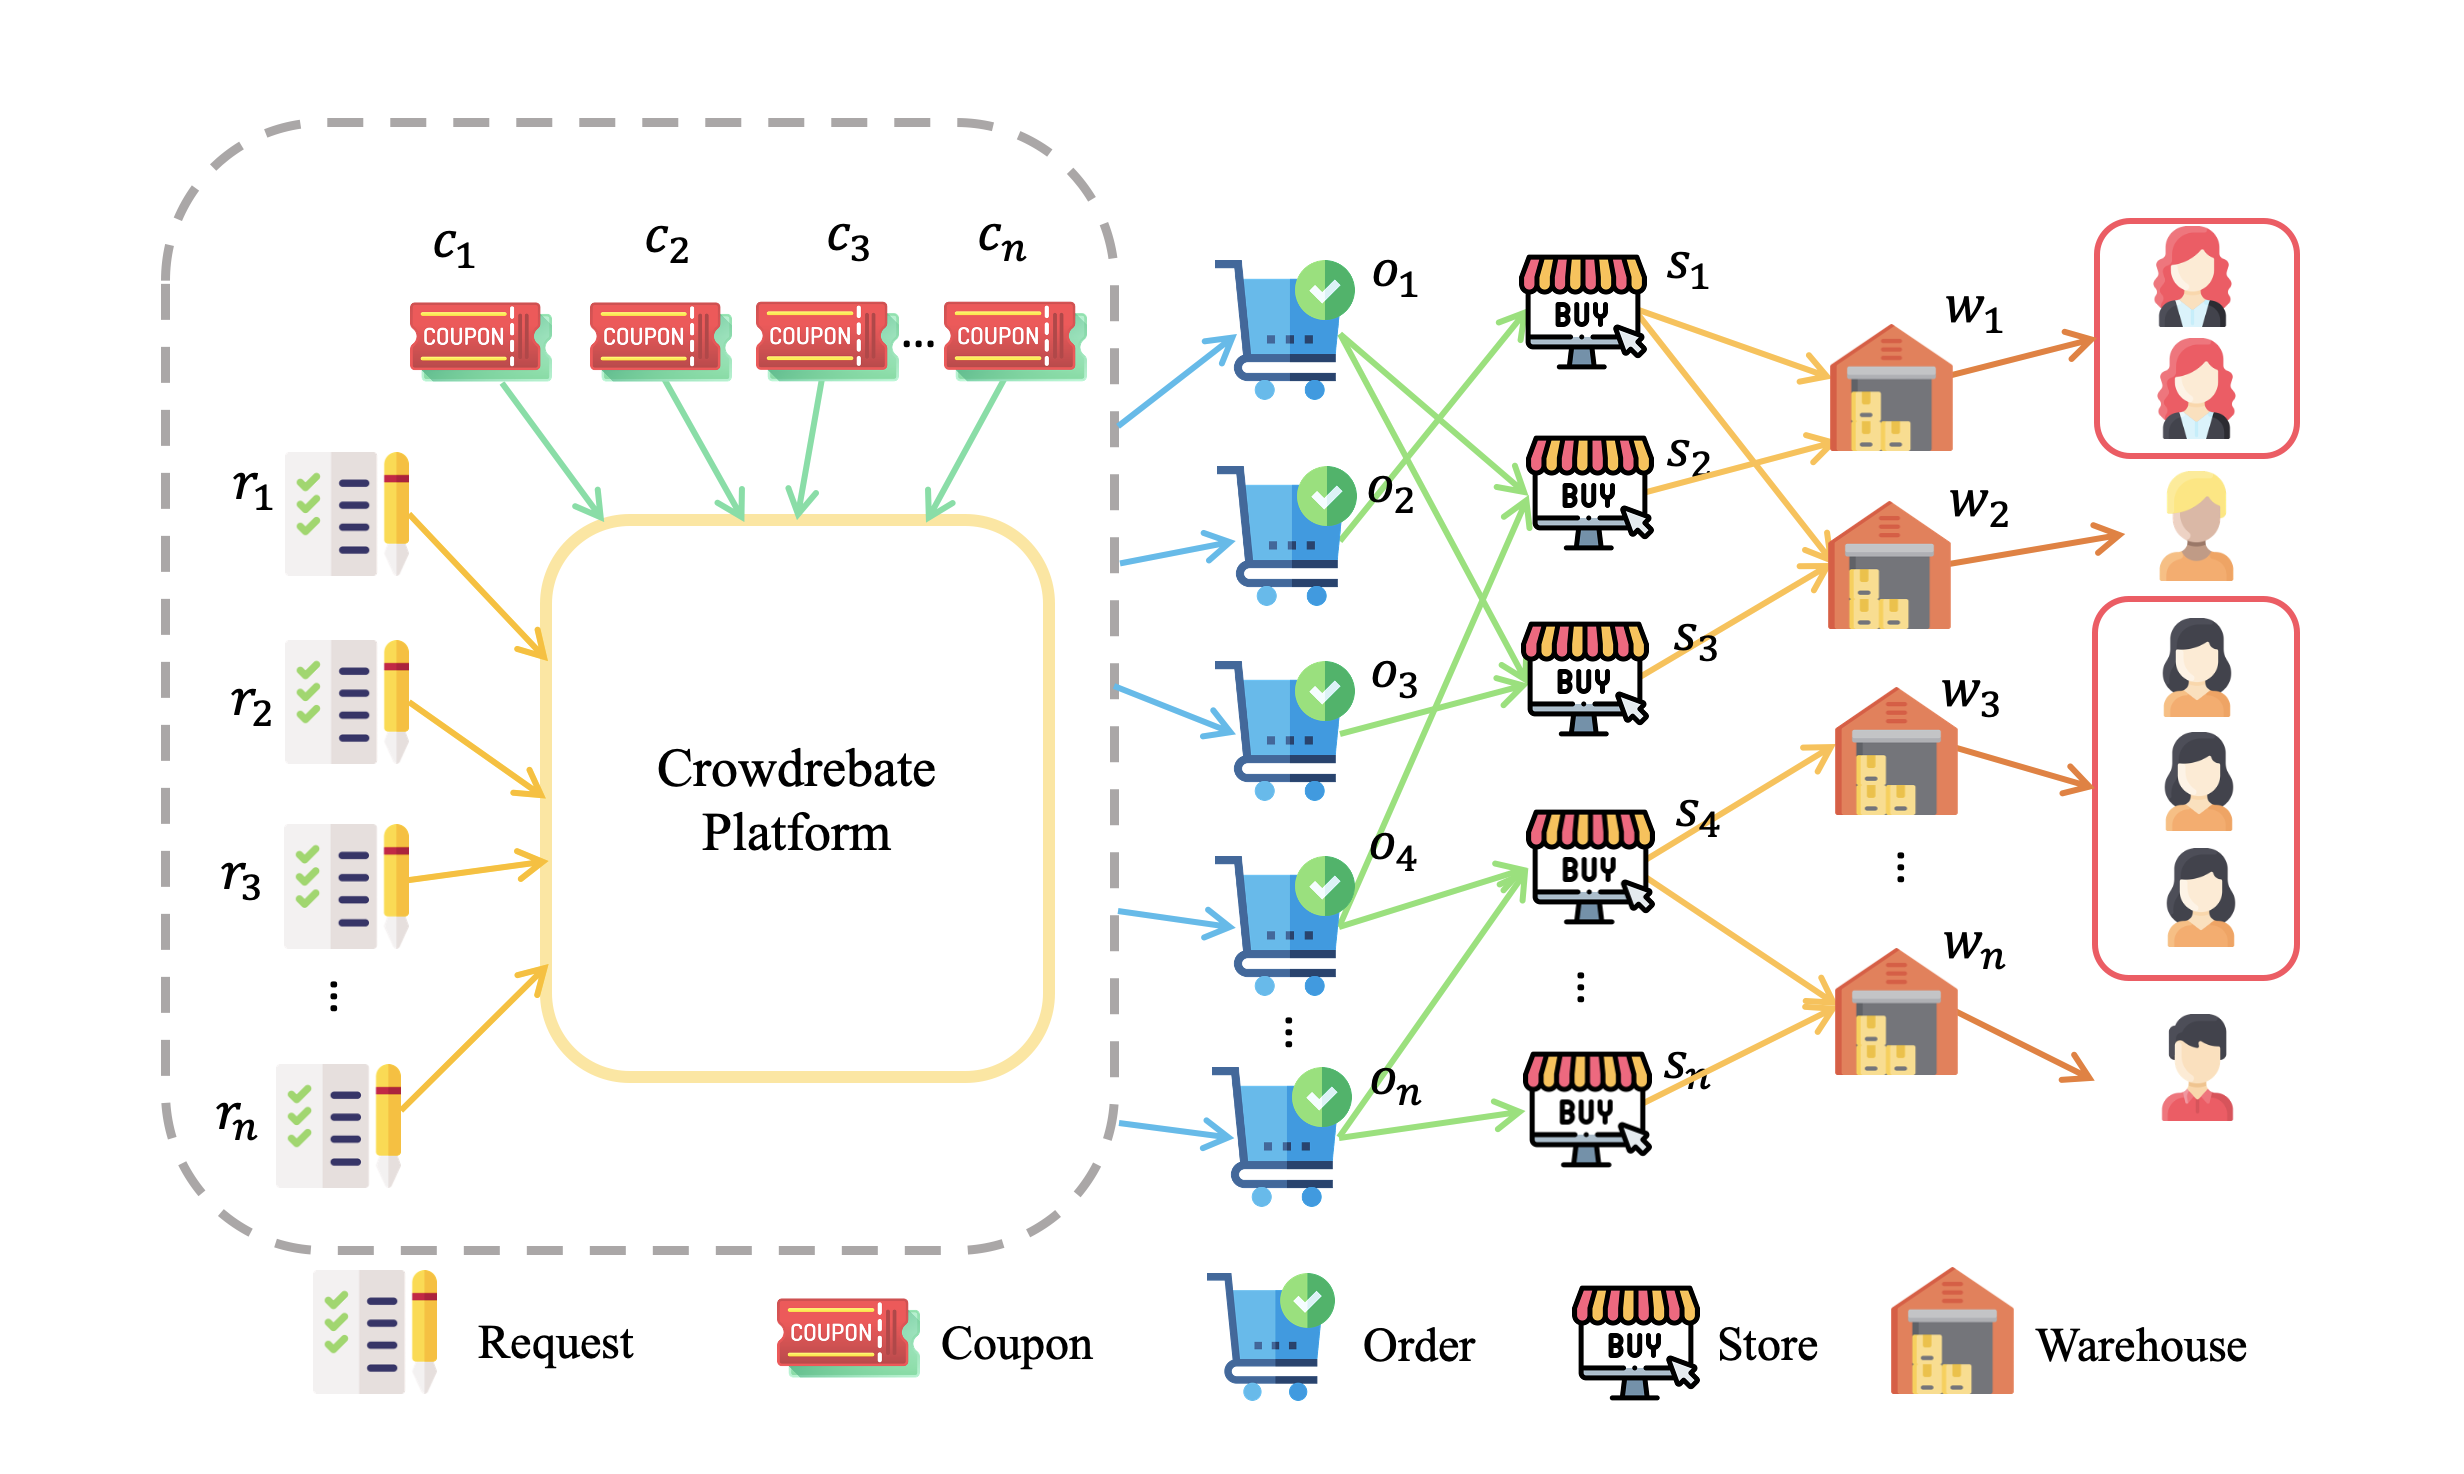
\includegraphics[width=0.4\textwidth]{../figure/crowdrebate process.png} %插入图片,[]中设置图片大小,{}中是图片文件名
	\caption{The operation process of crowdrebate} %最终文档中希望显示的图片标题
	\label{fig:Crowdrebate} %用于文内引用的标签
	\end{figure}

Under these circumstances, our demo-Crowdrebate firmly grasps consumer's pain point. Crowdrebate collects users’
purchasing requests and group their requests into orders to
maximize total benefit. Meanwhile, we give the exposure of online retailers' promotions so that more users would participate in promotions. To summarize, not only do we dedicate ourselves to help users get more benefits, we also devote ourselves to help e-commerce platforms fill more orders, increase platforms’ revenue, and ultimately achieve a bilateral win-win situation.

Our platform operates as follows~\ref{fig:Crowdrebate}. Users can post their requirements on our platform. Each requirement corresponds to the e-commerce platform they would like to order from, such as the specific stores, specific products, and prices, as well as the expected period of placing order. Based on the received requests, we will make an order association and match the coupons we crawled from the e-commerce platform to maximize each order's rebate. Owing to the fact that we place the orders for consumers, the products will first be sent to our warehouses from the online stores, and then we will distribute the products to the according users.

Generally, Crowdrebate relies on three components. The user interface provides service for users to post requests and track datas. The algorithm library supports our core features, group ordering and recommendation. The data manager handles business logic and data storage.

Thus, our demo has following contributions:
\begin{itemize}
	\item We develope a platform for users to post for group ordering and track realtime information on mobile phones.
	\item We design two algorithms to combine orders for maximum rebates under different scenarios.
	\item We equip the platform with process automation and recommendation to handle large scale data and enrich user experience.
\end{itemize}
\begin{figure}[t] 
	\centering %图片居中
	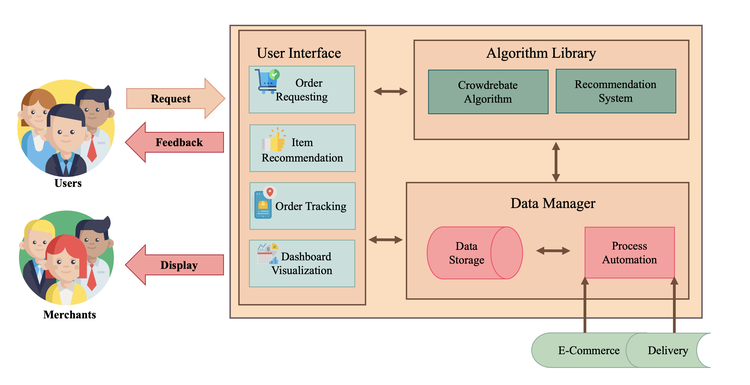
\includegraphics[width=0.4\textwidth]{../figure/ar.png} %插入图片,[]中设置图片大小,{}中是图片文件名
	\caption{The architecture of crowdrebate} %最终文档中希望显示的图片标题
	\label{fig:ar} %用于文内引用的标签
\end{figure}


\section{System Architecture}

Figure~\ref{fig:ar} depicts the architecture of Crowdrebate platform. The user interface module runs on the client-side, enabling both general users and merchant users to get corresponding services. The other three core modules, process automation, crowdrebate algorithm, and recommendation system, run on the server host and provide support for the core functionalities in Crowdrebate. We introduce the technical details of these modules in the rest part of this section.

\subsection{User Interface}

There are two types of users interacting with the user interface module, ``general users'' and ``merchant users''. General users, who seek group buying to meet the threshold of rebates, can request and track their orders with the interface while getting a personalized recommendation. Merchant users from online shopping platforms can benefit from the data dashboard to gain a better understanding of user portraits. This module consists of the following four functions.

\subsubsection{Order Requesting}

Users with the need for group shopping can post their requirements on Crowdrebate with this order requesting function. The input for this function consists of two parts, product information, and customer information. The former includes the shopping platform, product link, and promotion type, which help the web crawlers to target the specific item and its promotions. The critical part of customer information is expected time slots and delivery addresses, impacting the rounds and delivery costs for the crowdrebate algorithm to run.

\subsubsection{Order Tracking}

The order tracking function enables users to manage all historical orders. No matter whether one's item is waiting in the pool, being processed for a group order, or already on delivery, users can track real-time status for his order. Crowdrebate platform utilizes the web crawler, the crowdrebate algorithm, and the order bot to automate the process of group order and updates data timely for users to track.
	
\subsubsection{Item Recommendation}

The item recommendation functions show users products that best fit personal demands. Crowdrebate has top coupons and recommended products on the home page, where all users share the same information of top coupons while the recommended products are personalized. Both features are fed with data from Crowdrebate.

\subsubsection{Dashboard Visualization}

Crowdrebate opens API and provides a visualized data dashboard to cooperating online shopping platforms. With the visualized dashboard, merchant users can access to internal data depicting user portraits, product sales, and coupon popularity.

\subsection{Crowdrebate Algorithm}

Crowdrebate algorithm can place orders for users' best interests and works as one of the most crucial components in our platform. Considering the combination of coupons and delivery costs, Crowdrebate proposed two algorithms, the order-first algorithm and the delivery-first algorithm, to adapt to different scenarios. Users can freely choose from these algorithms which best fits their needs, and their requests will wait in two pools to process separately.

\textbf{The Order-First Algorithm.} In most cases, coupons with strict thresholds usually guarantee tempting rebates that should way cover the delivery costs. Under such a scenario, we propose the order-first algorithm to place orders. Generally speaking, this algorithm greedily packs orders for a maximum amount of total rebates while ignoring delivery costs. For each coupon, we traverse requests in the eligible pool and calculate the differential rebate amount when compared to placing an order separately, and the request with the largest amount will be integrated into one order until for any request the differential rebate amount fails to increase. However, the number of coupons used in a newly merged order may exceed the upper limit since their amounts are calculated separately before the merger. We introduce "Dif procedure" to tackle extra coupons while computing for the differential rebate. After packing requests, we need to place the order and assign one single address as the delivery destination. While this algorithm doesn't take the delivery into account before, it assigns a warehouse to the order to minimize the cost of delivery now.

\textbf{The Warehouse-First Algorithm.} The order-first algorithm performs well in most cases; however, it still suffers from two drawbacks. The first one is due to its lack of consideration for delivery costs, and once the delivery cost gets much higher, this algorithm performs poorly. The second defect results from the time complexity introduced by the error correction Dif procedure, which can be fatal when handling peak shopping festival traffic. As a result, a more efficient approach, the warehouse-first algorithm, is proposed to tackle the large scale data and non-negligible delivery costs. Instead of directly combining requests for higher rebates, we first group those requests sharing the same warehouse. Only then will we merge requests within the same warehouse for higher rebates. The preprocessing procedure divides the integral data set into smaller groups to constrain the batch size and running time, and grouping by delivery destination guarantees relatively small delivery costs. Basically, the warehouse-first algorithm is more efficient and can produce a better result for higher delivery costs, while the order-first algorithm stands out when rebates are profitable enough to cover delivery costs. Before users can freely choose from algorithms above, we run the order-first algorithm compulsorily for the cold start since the scale of requests is too small to be split and should handle the higher time complexity while bringing users more rebates.

\subsection{Process Automation}

Crowdrebate uses the process automation module to complete the whole procedure from picking items to pay for our server's orders. Basically, the module comprises two sub-modules, the web crawler retrieving the information of products and coupons, and the order bot to automatically place an order. 

\textbf{The Web Crawler.} Currently, two types of information will be crawled, respectively, products and coupons. For the product information, this module retrieves the data passively. Before the user can post a request, a URL linked to the product must be provided to activate the web crawler. With the pasted URL, the spider bot crawls the associated coupons along with the product information and will specifically return options like size or color for the user to choose. Besides, we crawl all the metadata of this product for further recommendation function. For the coupon information, this module actively seeks data. We take the initiative to crawl information from coupon websites like Etao~\cite{etao} to enrich our available coupon pools. 

\textbf{The Order Bot.} The crowdrebate algorithm runs in rounds periodically and produces final grouped orders each round. Therefore we develop the order bot to handle those orders automatically. Since some exclusive coupons in different orders may violate each other, we introduce multiple accounts to place those exclusive orders, enabling us to run the scripts in parallel.

\subsection{Recommendation System}

The recommendation system module is one of the critical features of Crowdrebate. Considering the online shopping scenario, there will not be a massive change for items on sale. The similarity of items is relatively stable to the user’s interest, so we adapt the item-based collaborative filtering~\cite{sarwar2001item} to recommend similar products. The recommendation system is built upon metadata from the web crawler and users’ historical requests and ratings. Since users on Crowdrebate pursue higher rebates, we improved the algorithm to rank on rebate amounts instead of similarities to meet their demands better. 
\section{Demonstration overview}

In this section, we describe different kinds of scenarios that users commonly encountered in the Crowdrebate platform, which include a new request submission, top deals and products viewing, status checking, and data analyses.

\subsection{Scenarios 1: Set up request}

\begin{figure}[t!] \vspace{-1ex}
	\subfigure[][{Set up a request}]{
		\scalebox{0.09}[0.09]{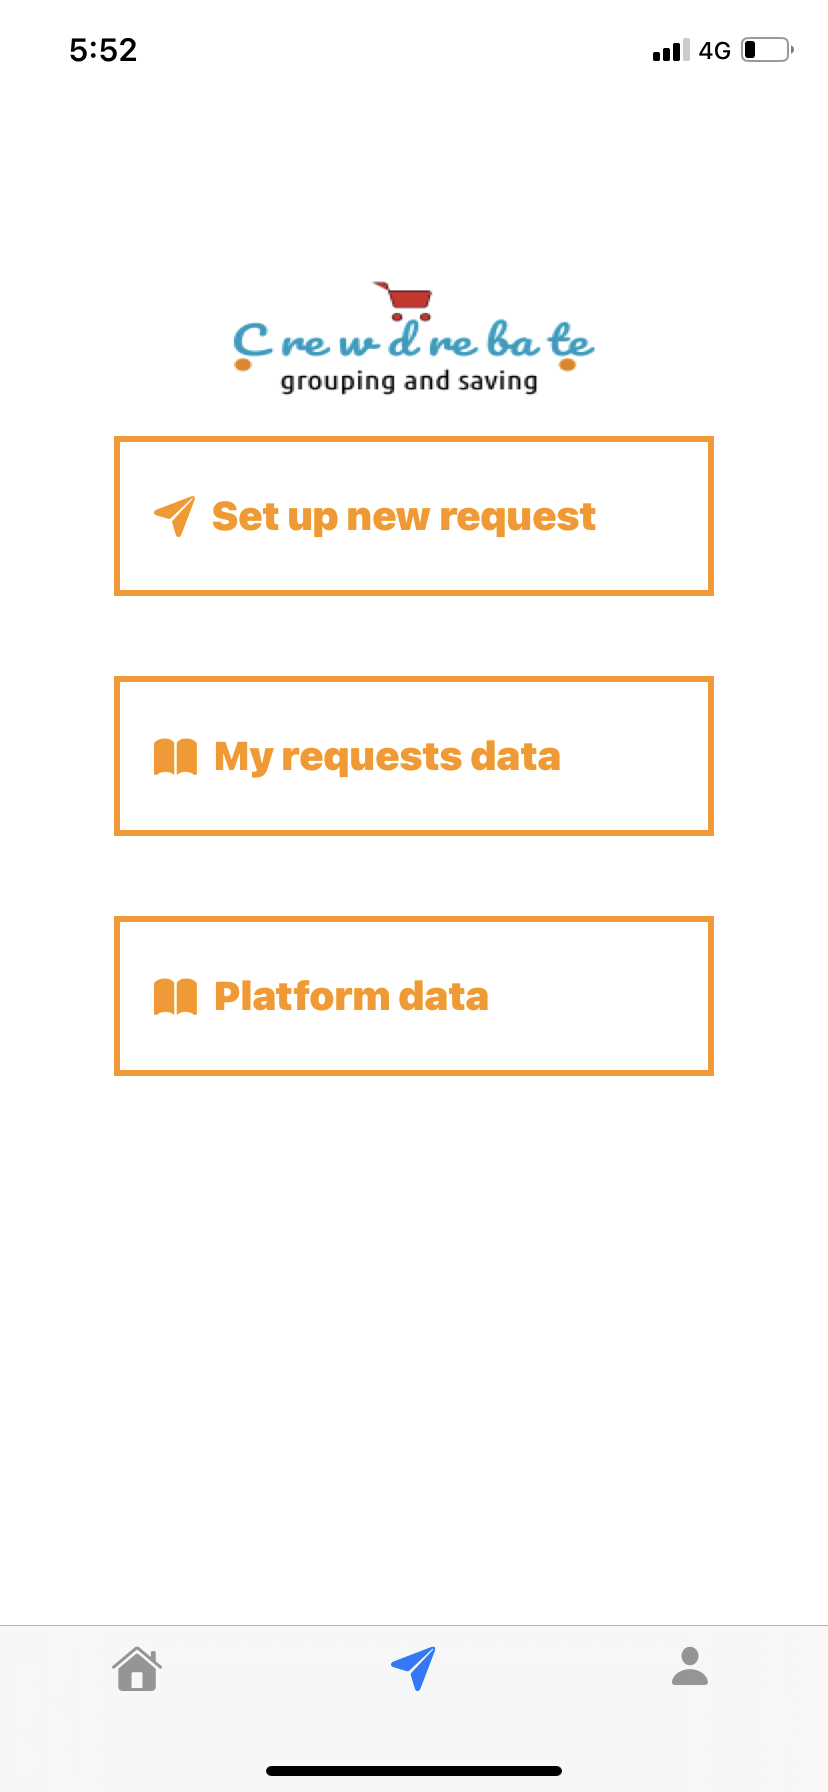
\includegraphics{../figure/request 1.png}}
		\label{fig:request1}}
	\subfigure[][{Fill in information}]{
		\scalebox{0.09}[0.09]{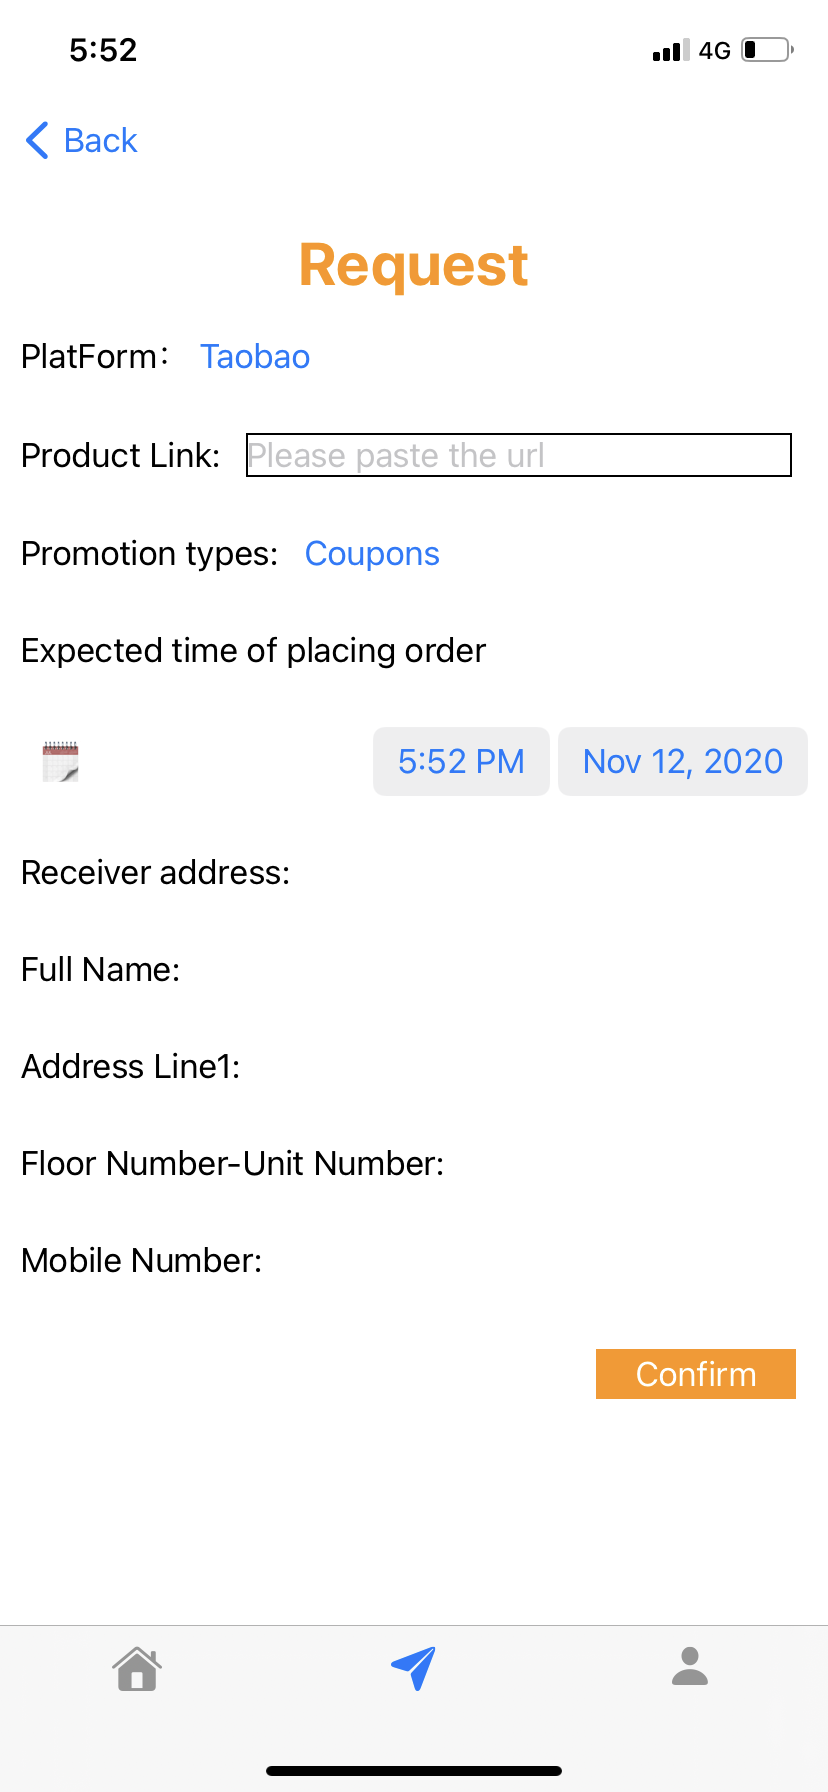
\includegraphics{../figure/request 2.png}}
		\label{fig:request2}}
	\subfigure[][{Information confirm}]{
		\scalebox{0.09}[0.09]{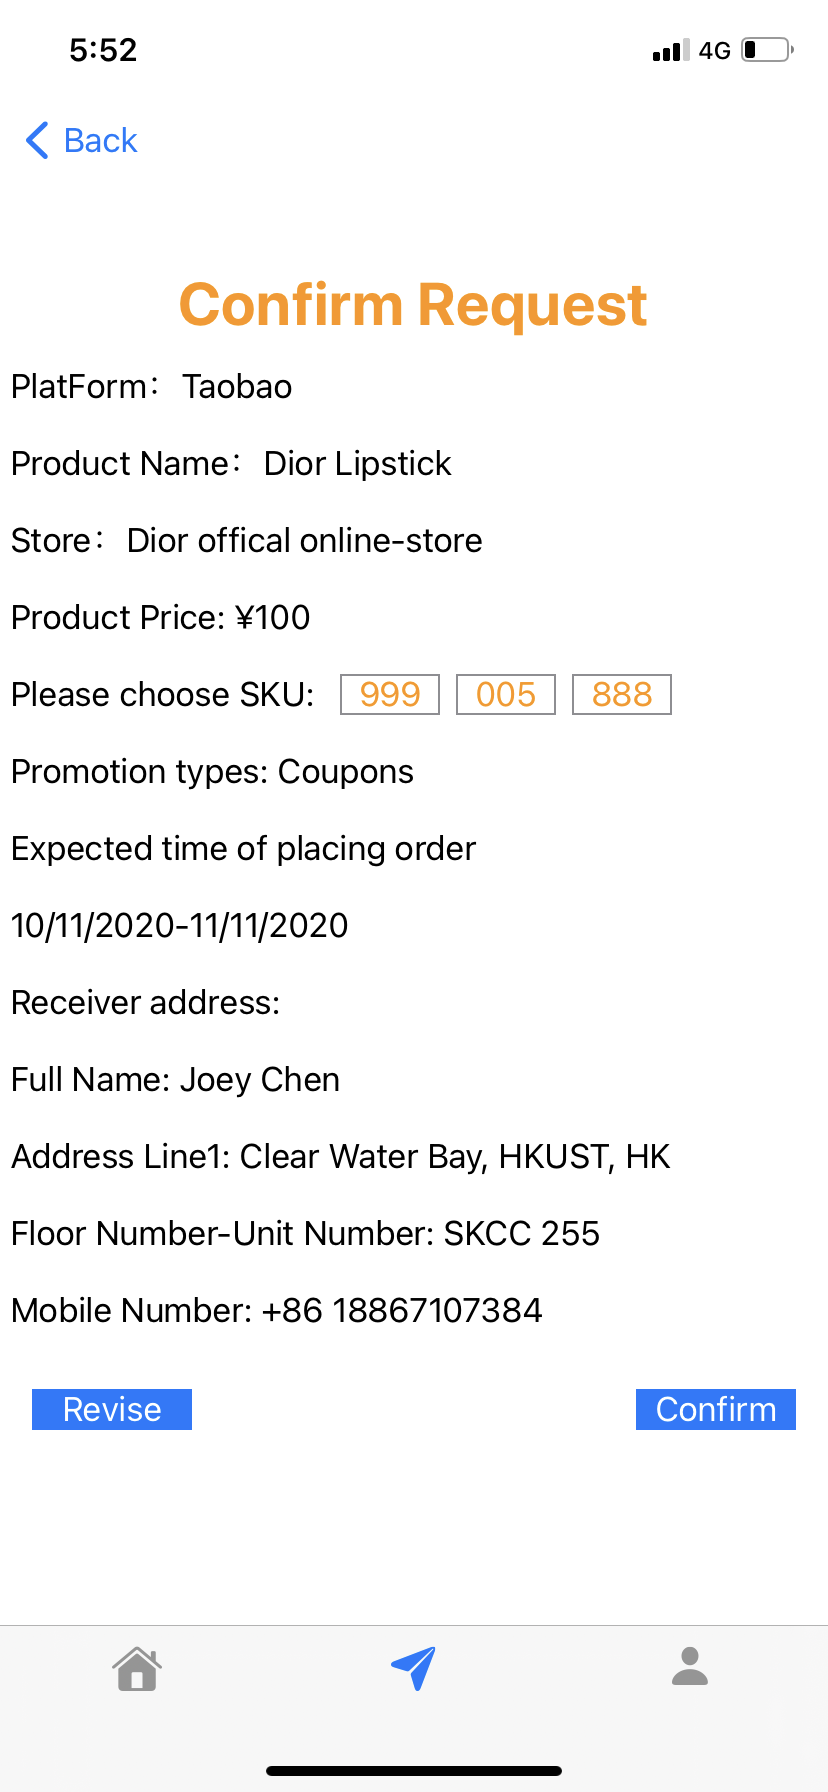
\includegraphics{../figure/request 3.png}}
		\label{fig:request3}}
	\caption{The flowchart of ``Set up a request''.}\vspace{-3ex}
	\label{fig:motivation}
\end{figure}

\textbf{As a regular user} completes the registration on our platform, has the certain product wants to buy, and clicks on the \textbf{Set up new request} button~\ref{fig:request1}, she/he will enter the page which guides her/him to fill in the following information~\ref{fig:request2}. The user needs to select the e-commerce platform he wishes to order from. In order to simplify the user's task and to prevent the platform from placing the wrong order of product, the user will need to copy the URL link of the product he wants to buy, and the platform will automatically crawl the product information such as price, store, promotions, etc. If there is more than one Stock Keeping Unit SKU for the product, we will also crawl to all the SKU information and ask the user to make a choice. Next, the user needs to select the type of promotions he wants to participate in, such as whether to enjoy the coupons or to receive more free samples, and the time slot she/he wants the platform to place the order. Finally, the user fills in the delivery address. After confirming the final information twice~\ref{fig:request3}, the platform will start to complete the request at the time specified by the user.

\subsection{Scenarios 2: Check my request data}

\begin{figure}[t!] \vspace{-1ex}
	\subfigure[][{Status of requests}]{
		\scalebox{0.13}[0.13]{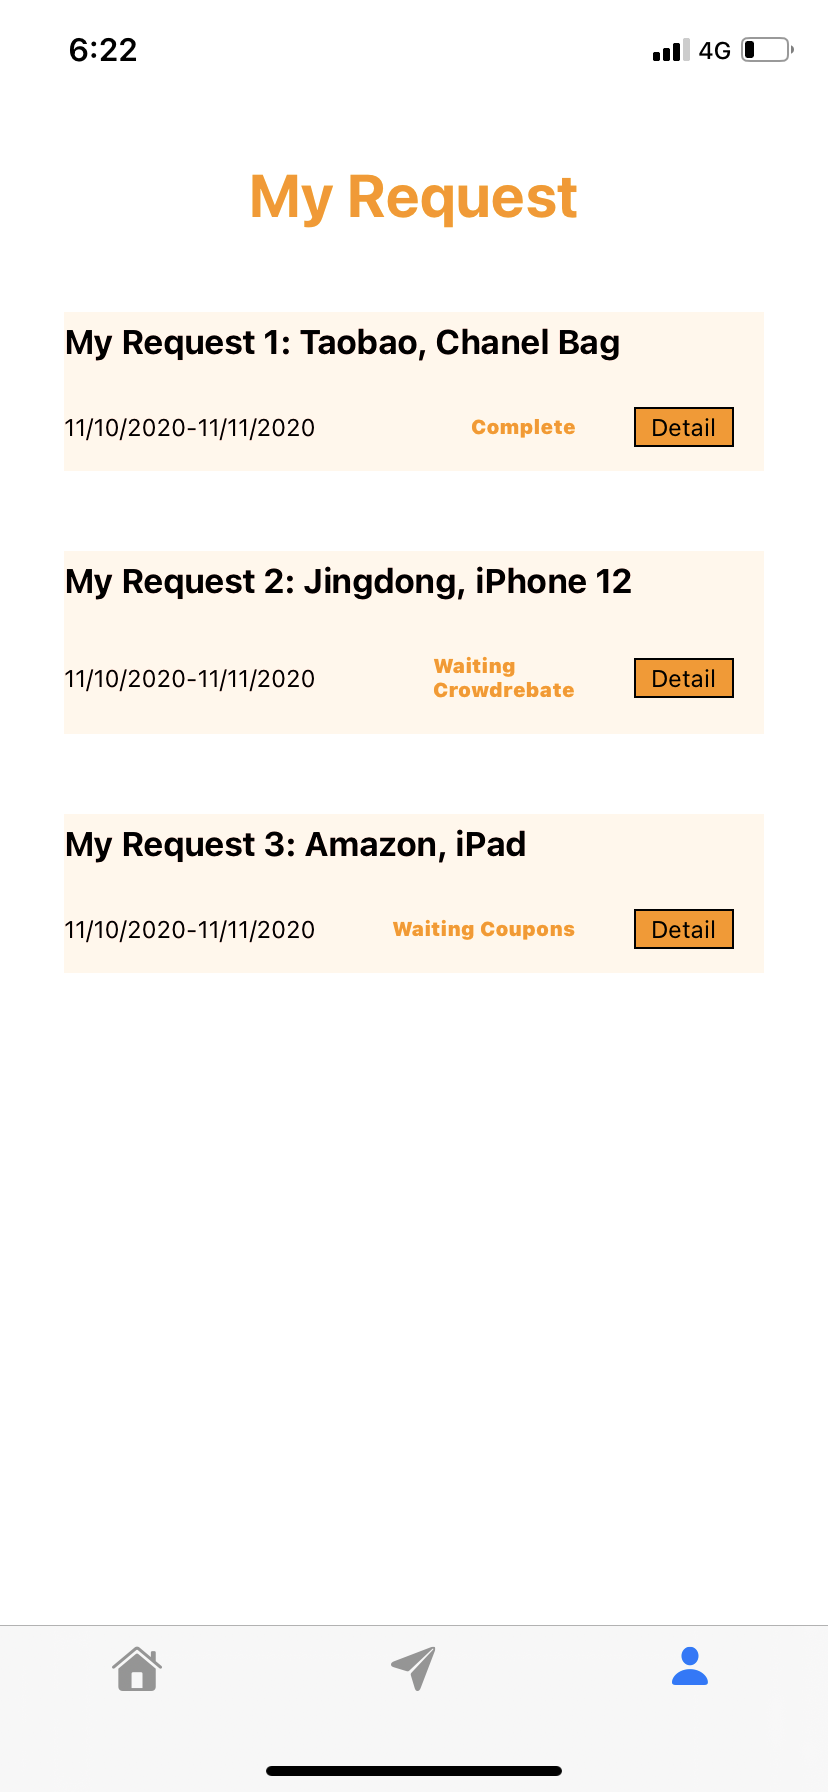
\includegraphics{../figure/check 1.png}}
		\label{fig:check1}}
	\subfigure[][{Personal data}]{
		\scalebox{0.13}[0.13]{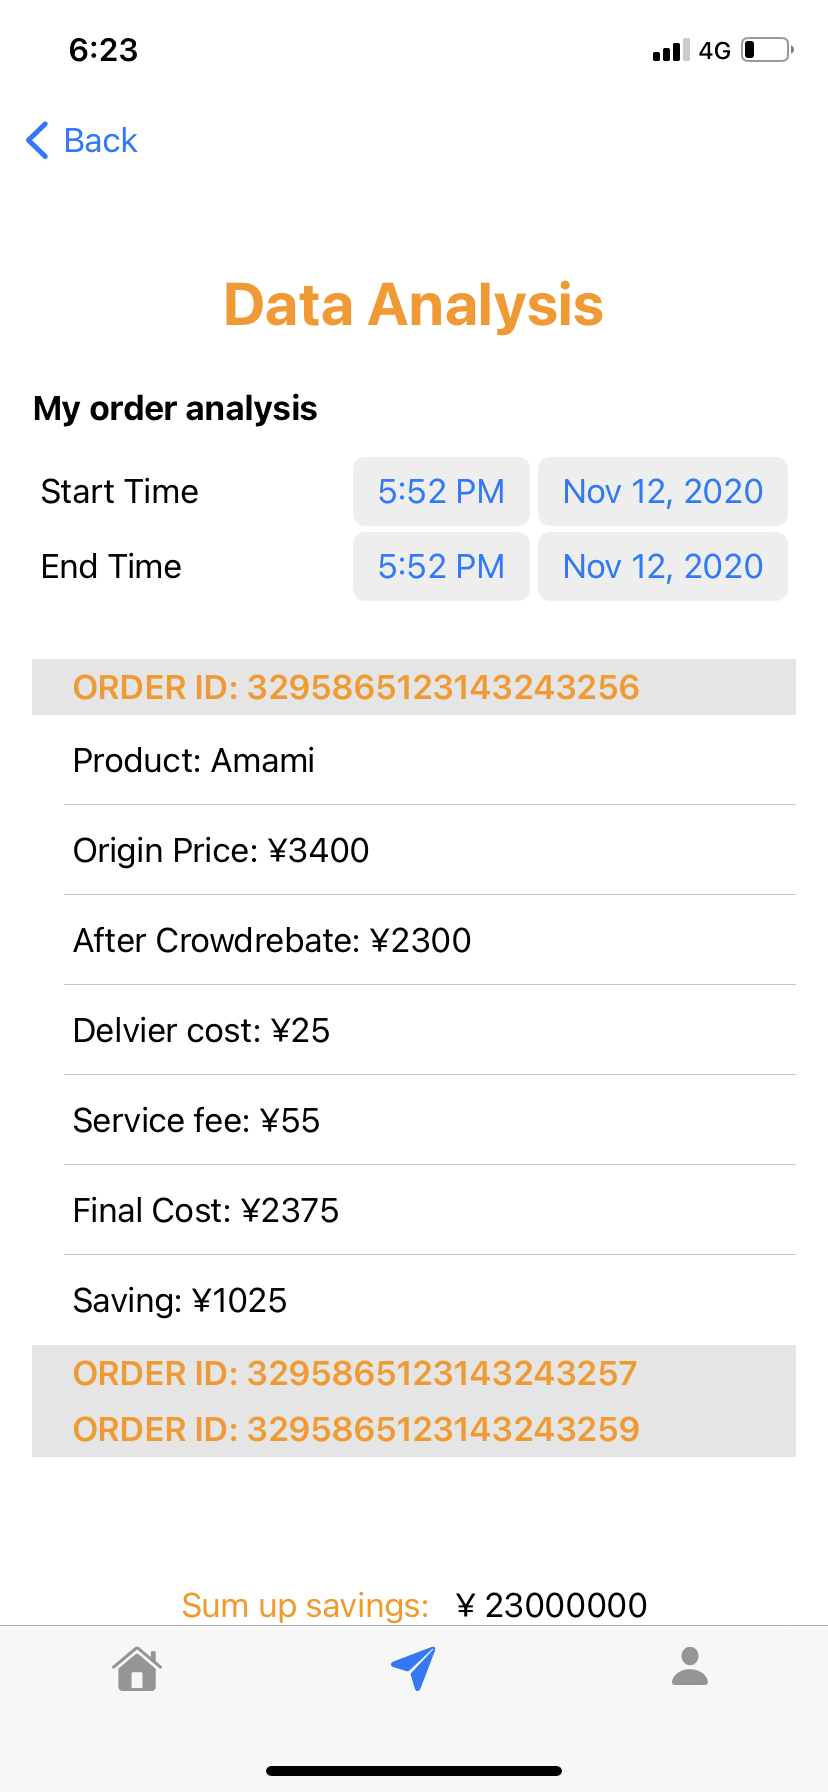
\includegraphics{../figure/check 2.png}}
		\label{fig:check2}}
	\caption{View status of requests and personal data".}\vspace{-3ex}
	\label{fig:check}
\end{figure}

After completing to set up a request, the user can check all the requests he/ she made on our platform on the personal page~\ref{fig:check1} and the status of each request, such as whether the order has been placed, and whether the product has been sent to the warehouse, etc.

Note that, if the user is interesting about the data of order, she/he can also see specific data for each request in the My request data page~\ref{fig:check2}, like the original price, the price after the platform placed an order for them, the shipping cost, the platform's service charge, and the saving after deducting various costs. The user also can choose to see the sum of the data over a period of time.

\subsection{Scenarios 3: View Top deals and top products}

\begin{figure}[t!] \vspace{-1ex}
	\subfigure[][{Today's deals}]{
		\scalebox{0.13}[0.13]{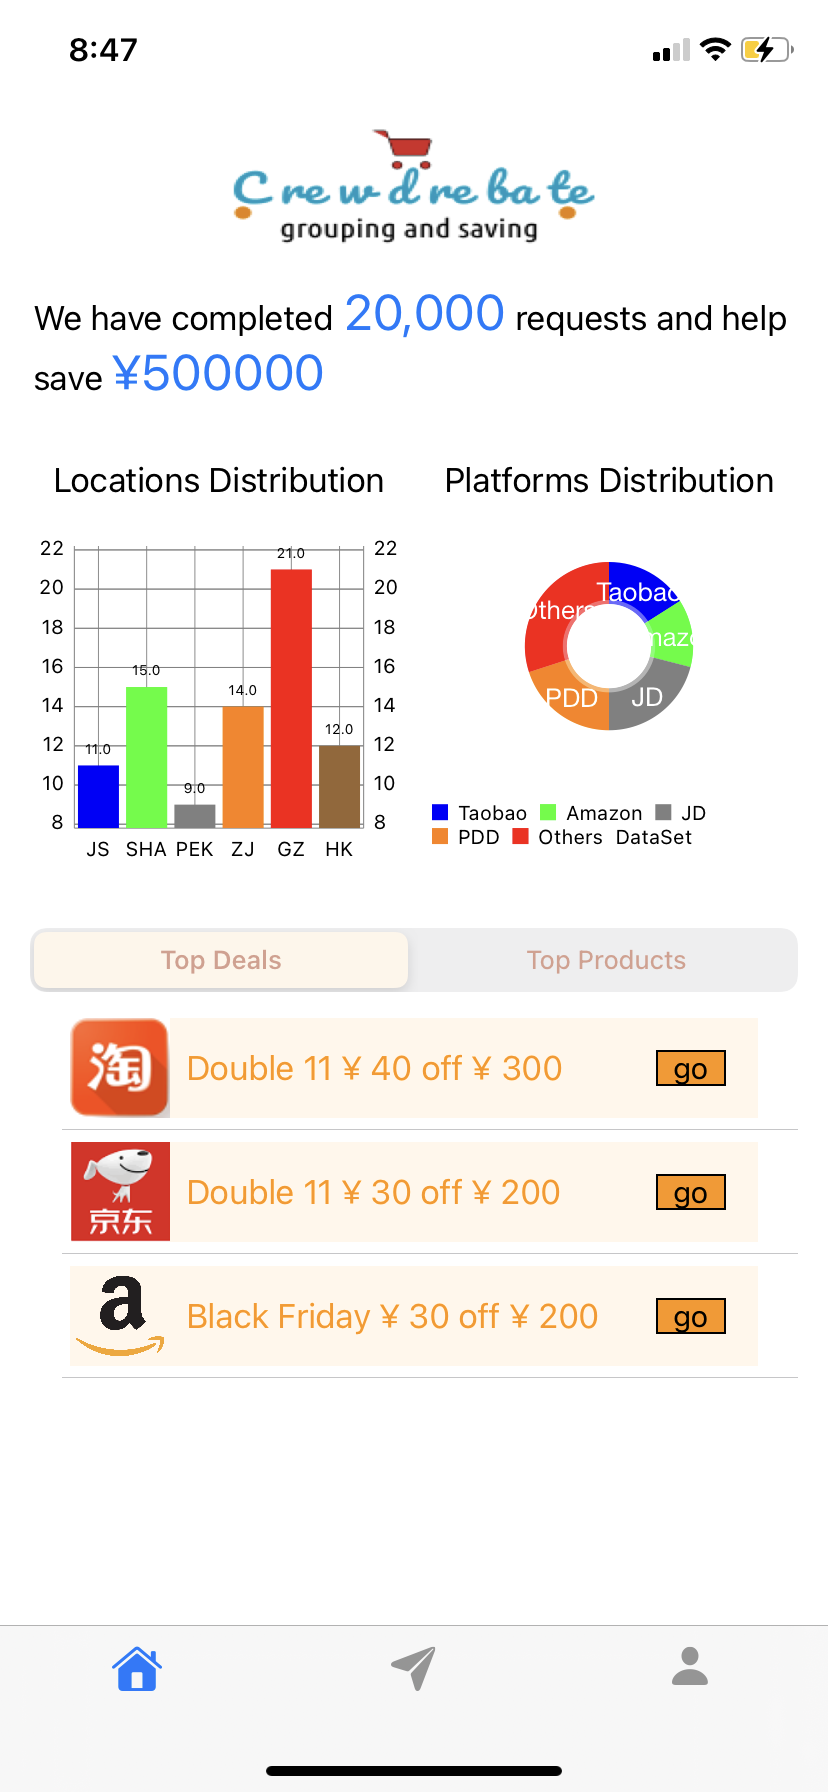
\includegraphics{../figure/home1.png}}
		\label{fig:home1}}
	\subfigure[][{Personalized recommendations}]{
		\scalebox{0.13}[0.13]{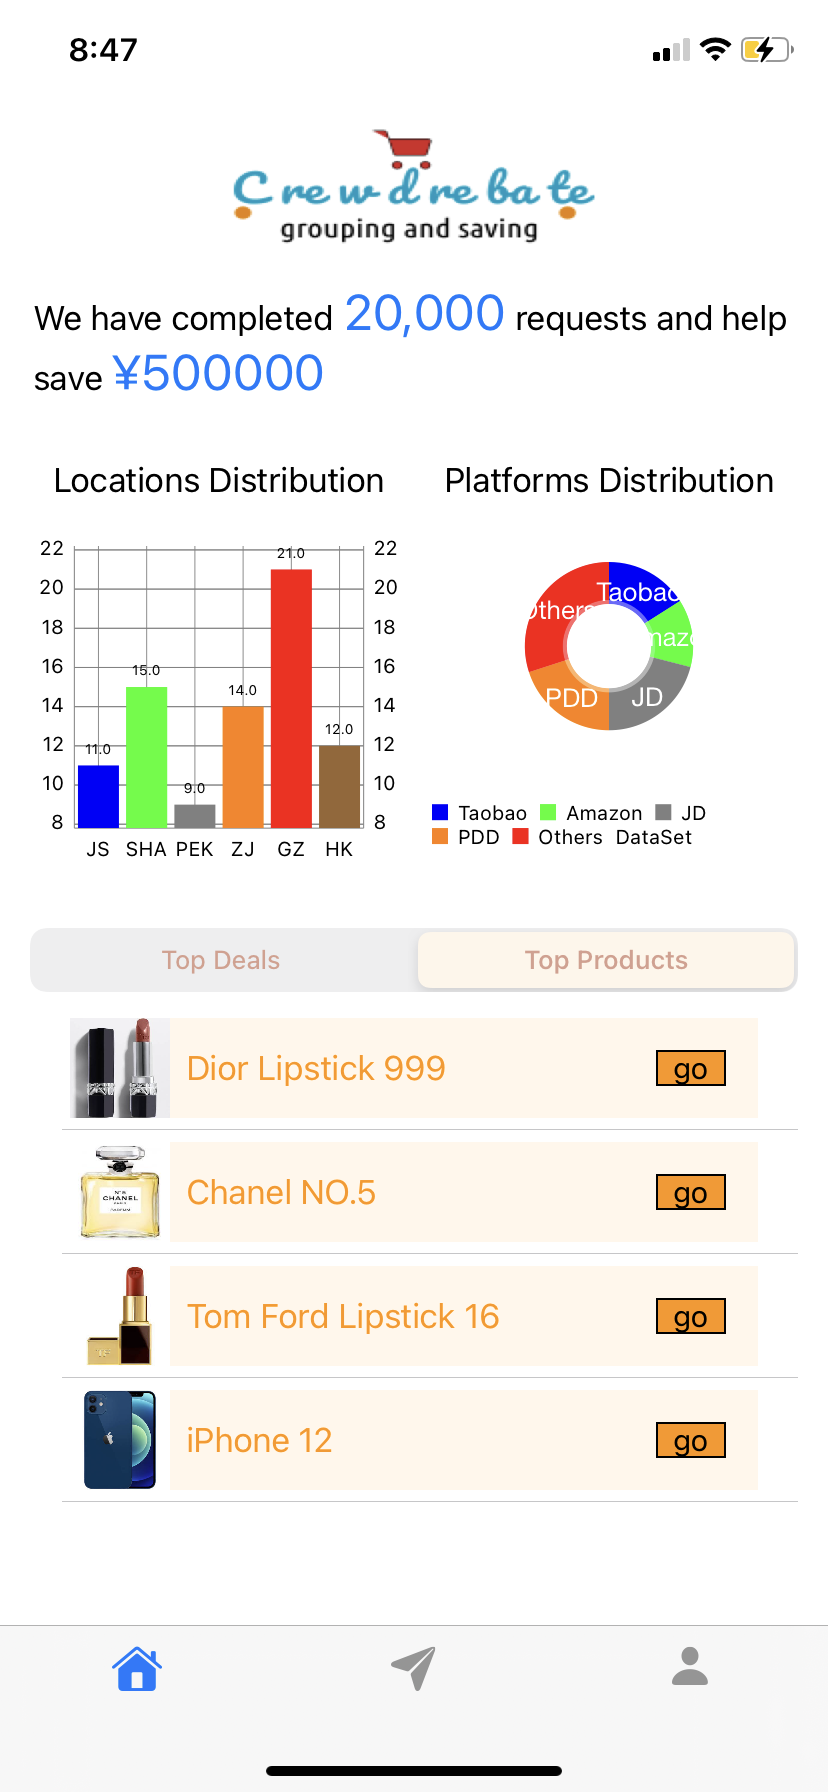
\includegraphics{../figure/home2.png}}
		\label{fig:home2}}
	\caption{View Today's deals and personalized recommendations.}\vspace{-3ex}
	\label{fig:home}
\end{figure}
When user are not sure about recent promotions of e-commerce platforms, she/he can use the home page to see our daily updates of platforms' top deals to save time~\ref{fig:home1}. When user has no clear shopping target, the platform will make personalized recommendations based on the previous purchase data~\ref{fig:home2}.

\subsection{Scenarios 4: Dashboard of data}

\textbf{As teammates} of the Crowdrebate platform or \textbf{Our cooperation partners}, in addition to the basic operations mentioned above, they can also carry out the following functions:

\begin{figure}[t!] \vspace{-1ex}
	\subfigure[][{Dashboard of crowdrebate data}]{
		\scalebox{0.13}[0.13]{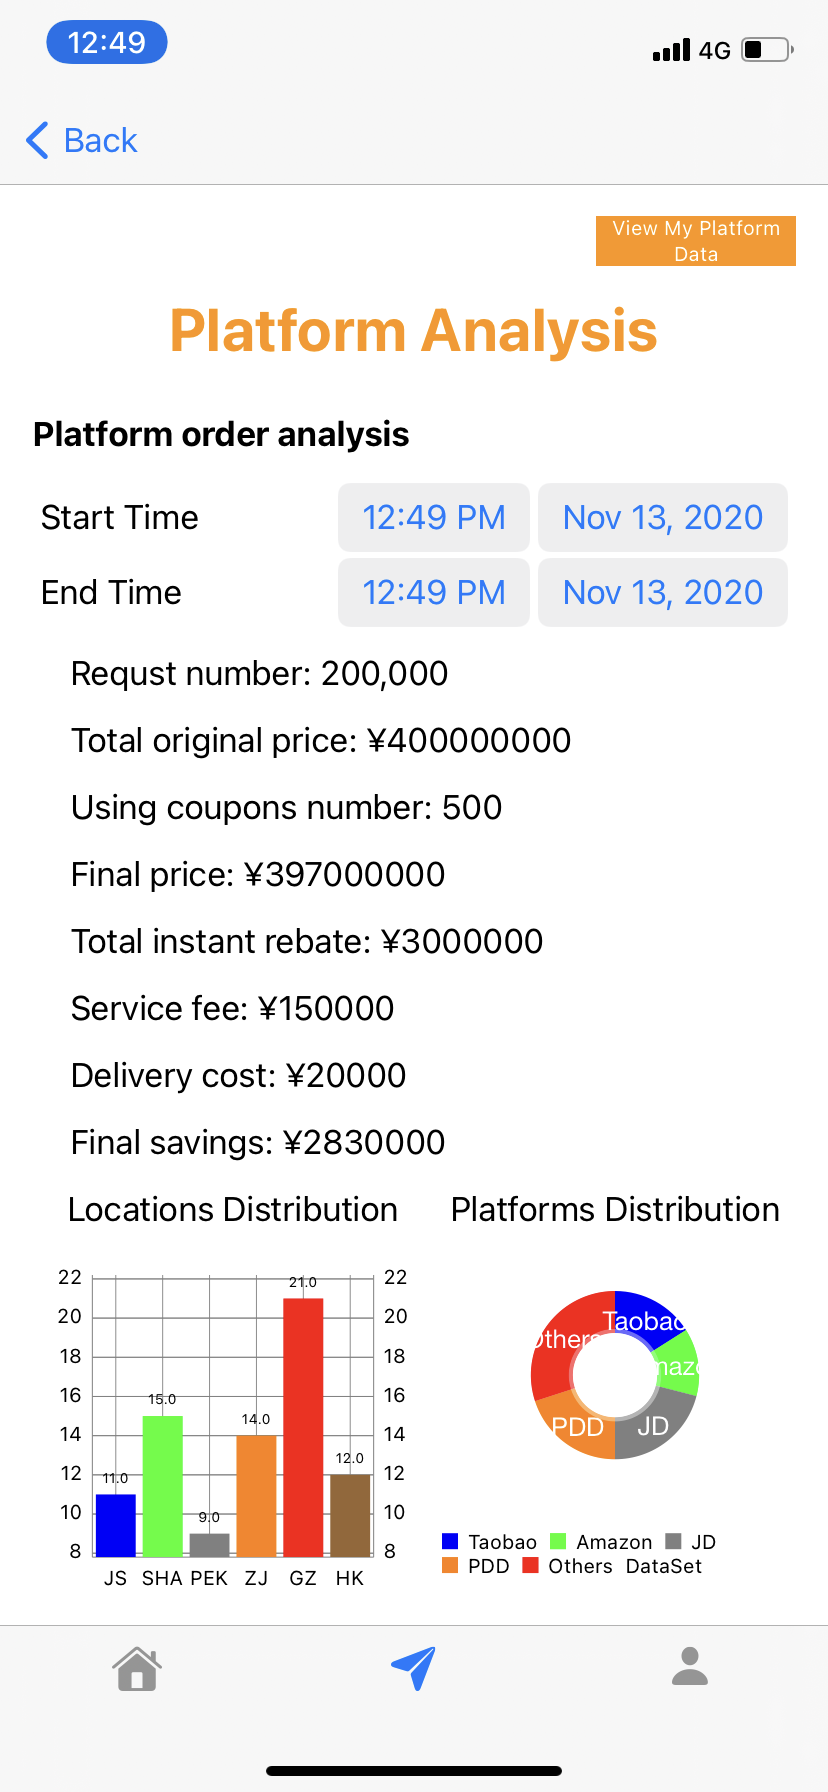
\includegraphics{../figure/data1.png}}
		\label{fig:data1}}
	\subfigure[][{Dashboard of cooperator data}]{
		\scalebox{0.13}[0.13]{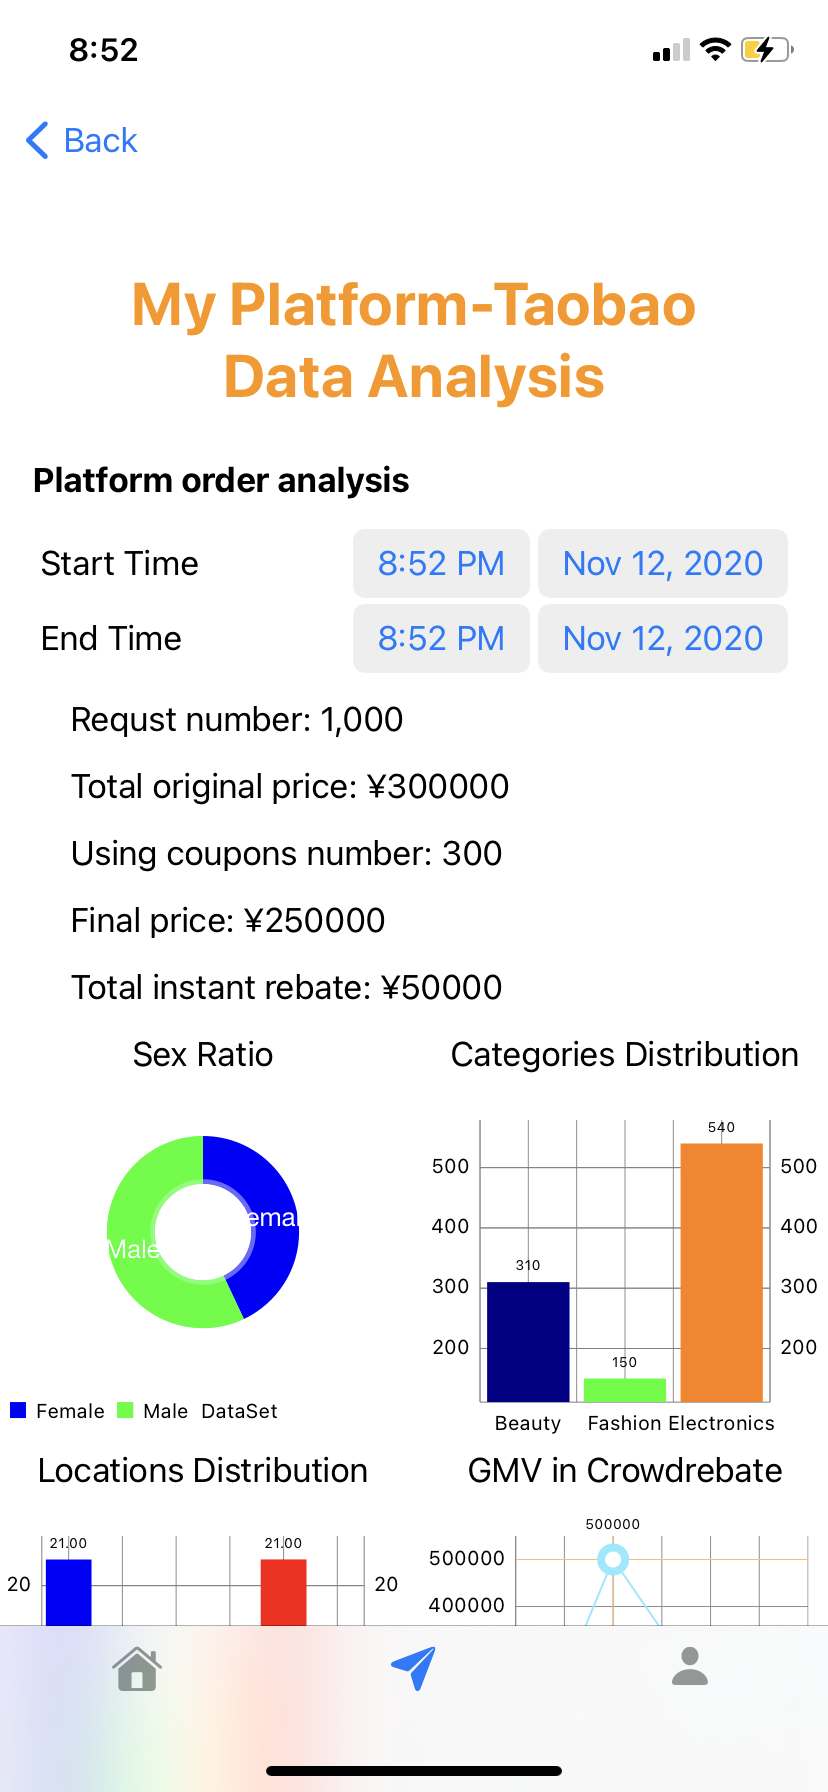
\includegraphics{../figure/data2.png}}
		\label{fig:data2}}
	\caption{Dashboard of data.}\vspace{-3ex}
	\label{data}
\end{figure}

Without being interfered with the user privacy, our platform staffs can enter the third button Platform data~\ref{fig:request1}, where they will be able to see a dashboard of data related to the whole platform, such as how many orders we have received, how many coupons we have used, how much money we have helped users to save, the distribution of our users by regions, and the distribution of platforms they like to launch request~\ref{fig:data1}.

As for our cooperation partners of e-commerce platforms, they can see a dashboard of data related to their platforms. For example, as Taobao cooperators, they can see how many of the requests initiated by our platform users are from Taobao, the distribution of categories they like to buy, the ratio of sex, etc~\ref{fig:data2}. This dashboard of data will help our partners to gain a more practical understanding of user preferences, design coupons, and reach a win-win collaboration mechanism.

\section{Conclusion}\vspace{-1ex}
\label{sec:conclusion}

In this demo, we will present the Crowdrebate platform, which collects requests from users, group requests into a set of orders to get more rebates, and relay products to different receivers in an order. We introduce the sketch of system architecture and demonstrate scenarios via several case analysis. 
 
 \vspace{-1.5ex}
%\section{acknowledgment}
\label{sec:ack}

If you think that this template helped you on writing research papers and you work on the related topics, please help to cite some of my publications 
\cite{cheng2016task, cheng2017utility, chen2014gmission, cheng2015reliable,  cheng2017prediction, chen2018effective, cheng2018experimental, cheng2018frog, cheng2019cooperation, chen2019minimize}. Thanks a lot!



\balance




\bgroup\small
\bibliographystyle{ieeetr}
\let\xxx=\bibitem\def\bibitem{\par\vspace{0mm}\xxx} % % When you need space at the end, change 1 to 0, which can be your last chance!
\bibliography{../reference/add}
\egroup

\nobalance
\newpage



\end{document}
